\chapter[IMPLEMENTACION]{IMPLEMENTACIÓN}
En el capitulo anterior, un diagrama de bloques de una arquitectura recomendada.Puesto a que nuestra implementación que para una cantidad limitada de usuarios  y como asi también para no depender de componenetes propietarios o
de pago  realizamos algunos cambios a esta arquitectura a probechando la interoperavilidad de Rasa Open Source. 

\begin{figure}[h]
    \centering
    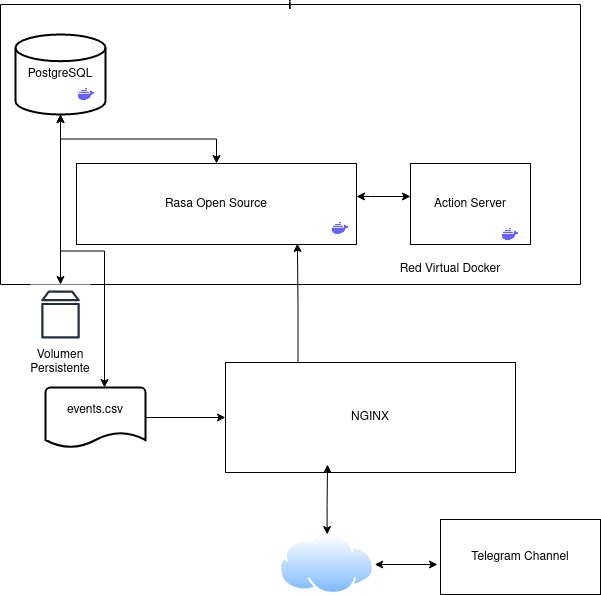
\includegraphics[width=\textwidth]{imagenes/cap4/server.png}
    \caption{Implementación Final}
    \label{fig:server_diagram}
\end{figure}


